\documentclass{beamer}
%
% Choose how your presentation looks.
%
% For more themes, color themes and font themes, see:
% http://deic.uab.es/~iblanes/beamer_gallery/index_by_theme.html
%
\mode<presentation>
{
  \usetheme{default}      % or try Darmstadt, Madrid, Warsaw, ...
  \usecolortheme{default} % or try albatross, beaver, crane, ...
  \usefonttheme{default}  % or try serif, structurebold, ...
  \setbeamertemplate{navigation symbols}{}
  \setbeamertemplate{caption}[numbered]
} 

\usepackage[english,russian]{babel}
\usepackage[utf8x]{inputenc}

\title[Your Short Title]{Отчет по второму заданию}
\author{Московченко, Абрамов,412 группа, Пантелеев, 411 группа}
\institute{МГУ им М.В. Ломоносова, Москва, Россия}
\date{2017\\Москва}

\begin{document}

\begin{frame}
  \titlepage
\end{frame}

% Uncomment these lines for an automatically generated outline.
%\begin{frame}{Outline}
%  \tableofcontents
%\end{frame}

\section{Introduction}

\begin{frame}{Цель}

\begin{itemize}
  \item Цель второго задания - проведение разведывательного анализа данных, чтобы опредедлить с каким поставщиком заключить договор.
\end{itemize}

\vskip 1cm

\end{frame}

\section{Some \LaTeX{} Examples}

\subsection{Tables and Figures}

\begin{frame}{Поэтапное описание разведывательного анализа данных}

\begin{itemize}

\item Происходит рассчет суммы всех мечей, произведенных каждой компании по отдельности. Из каждой полученной суммы вычитается количество сломаных мечей сумарно по всем кузнецам компании, в зависимости от партии. 
C помощью диаграммы размаха "Ящик с усами" проведен анализ эффективности производств каждой компании.
На диаграмме рахмаха изображена жирной линией медиана значений, выше - линия максимального значения для каждой компании и ниже - минимальное знчение.

\end{itemize}

\end{frame}

\subsection{Mathematics}

\begin{frame}{График}

\begin{figure}
            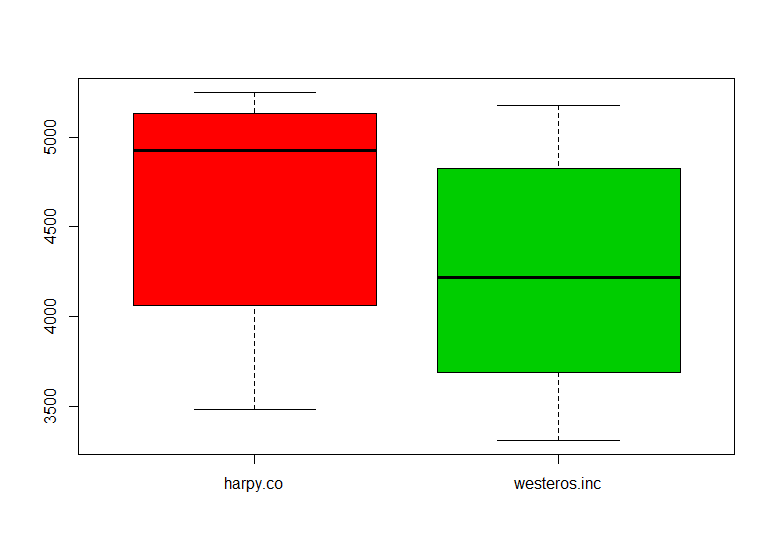
\includegraphics[width=100mm]{Rplot.png}
            \caption{"Диаграмма размаха Ящик с усами"}
            \label{Graph}

\end{figure}
\end{frame}


\begin{frame}{Поэтапное описание разведывательного анализа данных}

\begin{itemize}
\item После проведенного анализа можно прийти к выводу, что наиболее выгодно заключить контракт с компанией "Harpy.co". Так как контракт заключается на период 11 месяцев, следовательно необходимо смотреть по значению медианы. А медиана больше у компании  "Harpe.co"

\end{itemize}

\end{frame}

\begin{frame}{Задание выполняли}
      \begin{itemize}
            {\small
            \item Московченко Анастасия, студентка 412 группы. Написание презентации, написание кода.
            \item Пантелеев Игорь, студент 411 группы. Написание кода программы и анализ реультатов
            \item Абрамов Николай, студент 412 группы. Написание кода программы и анализ реультатов}
            \end{itemize}
  \end{frame}

\end{document}